\chapter{Instalación del calorímetro}
	El calorímetro originalmente era usado en la SLU (Universidad Sueca de Ciencias Agrícolas por sus siglas en sueco), en donde la red eléctrica es de 230 VAC. En Colombia se usan 110 VAC, razón por la cual una parte importante de la instalación del calorímetro consistió en configurar las entradas de voltaje del equipo para su operación en el país. Para esto fue necesario cambiar 2 fusibles por unos con capacidad para el doble de corriente, pues en los circuitos eléctricos con transformadores que permiten ajustar el voltaje de entrada, se tiene que conservar la potencia, la cual está dada por el producto de corriente y voltaje. Los fusibles se encuentran en el panel inferior derecho del calorímetro (\autoref{fig: fuseBox}), y en la parte trasera, los nuevos fusibles tienen valores de corriente de 4 A y 6 A, correspondientemente. Junto con este cambio fue necesario modificar las perillas selectoras de voltaje, una de las cuales se encuentra en el mismo panel del primer fusible (\autoref{fig: fuseBox}) mientras que el otro está en la parte trasera del módulo de control de la temperatura (\autoref{fig: decadeResistors}), el valor seleccionado es de 115 VAC.
	\begin{figure}[h]
		\centering
		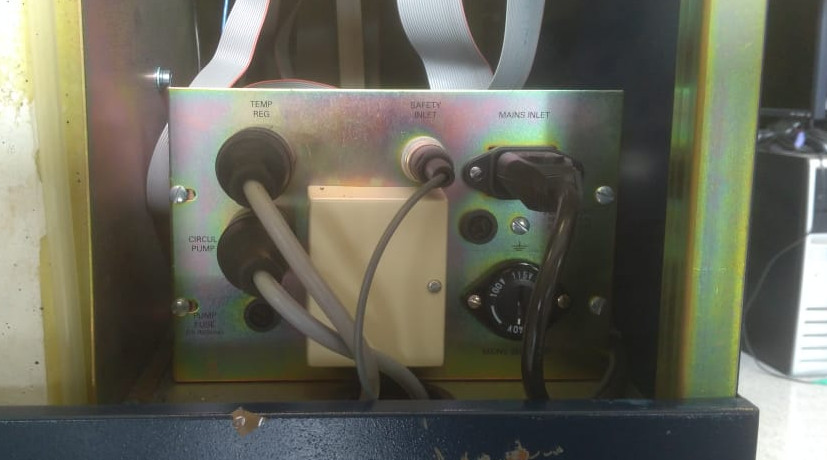
\includegraphics[width=0.7\linewidth]{Figures/fusepanel}
		\caption{Panel de selección de voltaje del calorímetro.}
		\label{fig: fuseBox}
	\end{figure}

	Posteriormente, uno de los cilindros de medición fue identificado en una de las cajas, se fijó al baño interno, y se llevaron a cabo las conexiones eléctricas con el módulo de amplificación como se muestra a continuación. 
	\begin{figure}[h]
		\centering
		\begin{subfigure}{0.24\linewidth}
			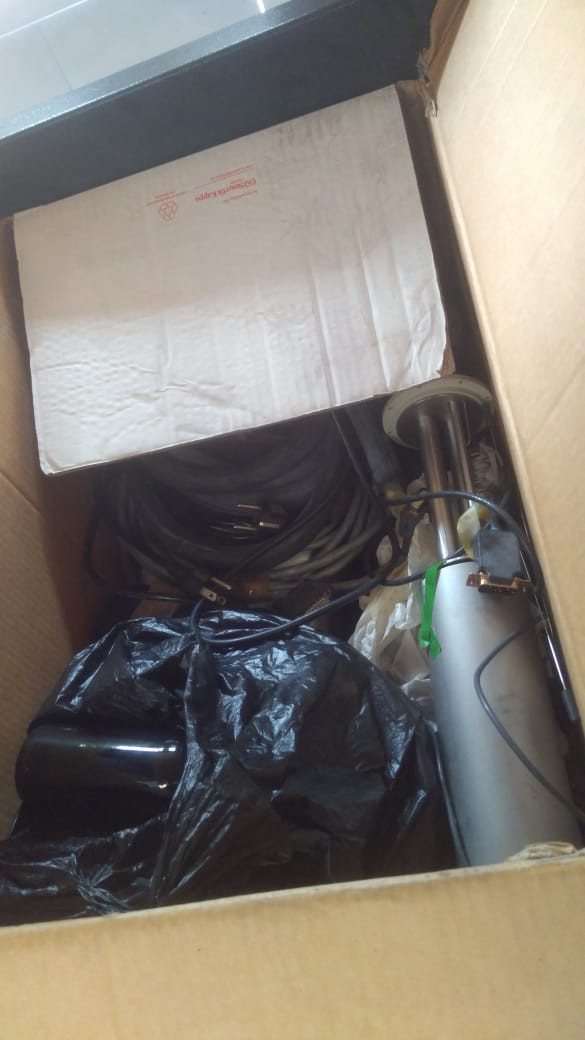
\includegraphics[width=\linewidth]{Figures/process/box1}
			\caption{ }
			\label{fig: subA}
		\end{subfigure}
		\begin{subfigure}{0.24\linewidth}
			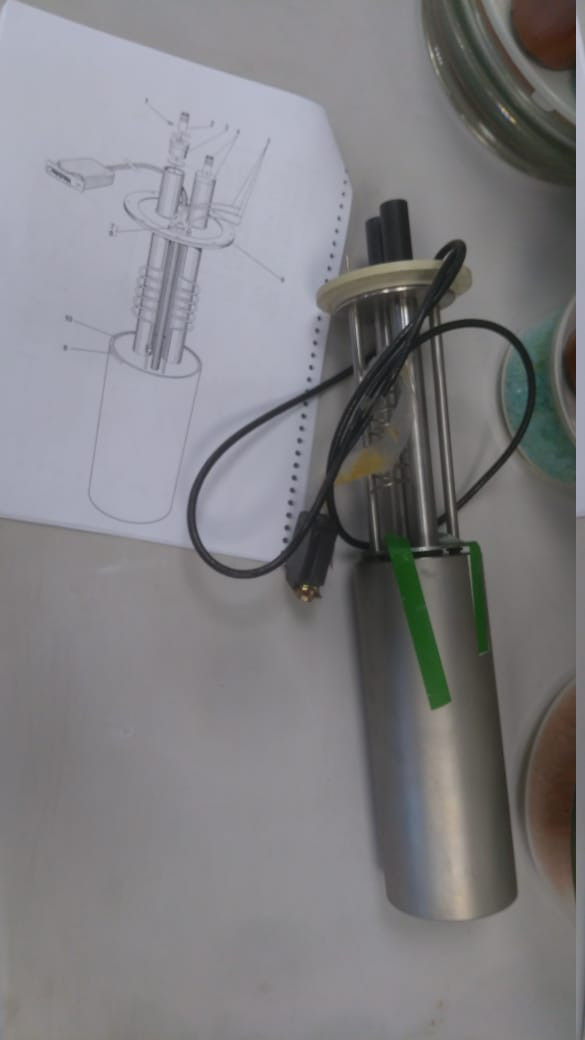
\includegraphics[width=\linewidth]{Figures/process/holder}
			\caption{ }
			\label{fig: subB}
		\end{subfigure}
		\begin{subfigure}{0.24\linewidth}
			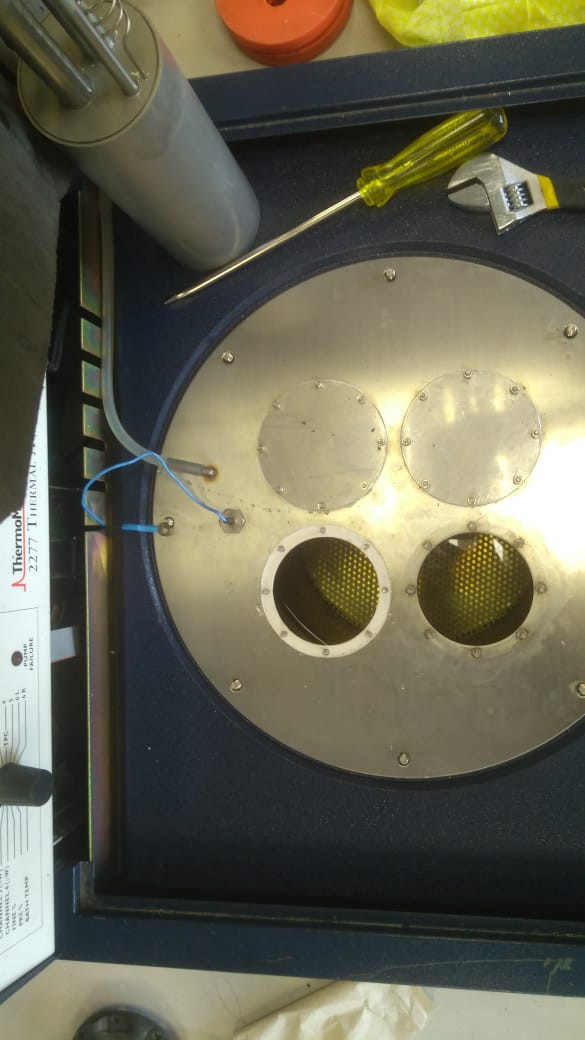
\includegraphics[width=\linewidth]{Figures/process/p1}
			\caption{ }
			\label{fig: subC}
		\end{subfigure}
		\begin{subfigure}{0.24\linewidth}
			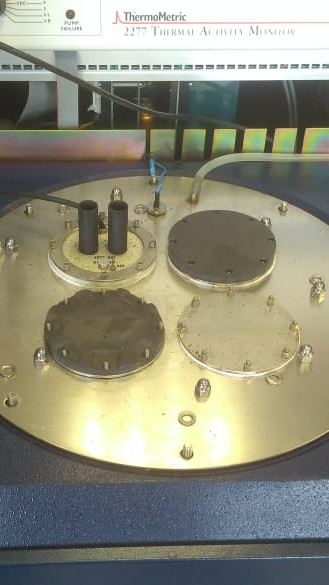
\includegraphics[width=\linewidth]{Figures/process/p2}
			\caption{ }
			\label{fig: subD}
		\end{subfigure}
		\begin{subfigure}{0.24\linewidth}
			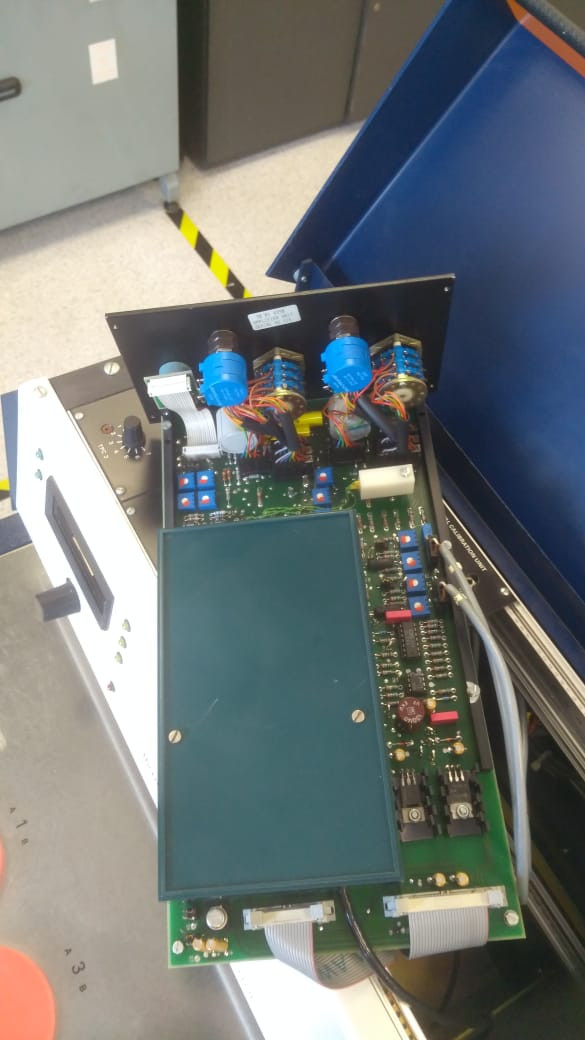
\includegraphics[width=\linewidth]{Figures/process/p3}
			\caption{ }
			\label{fig: subE}
		\end{subfigure}
		\begin{subfigure}{0.24\linewidth}
			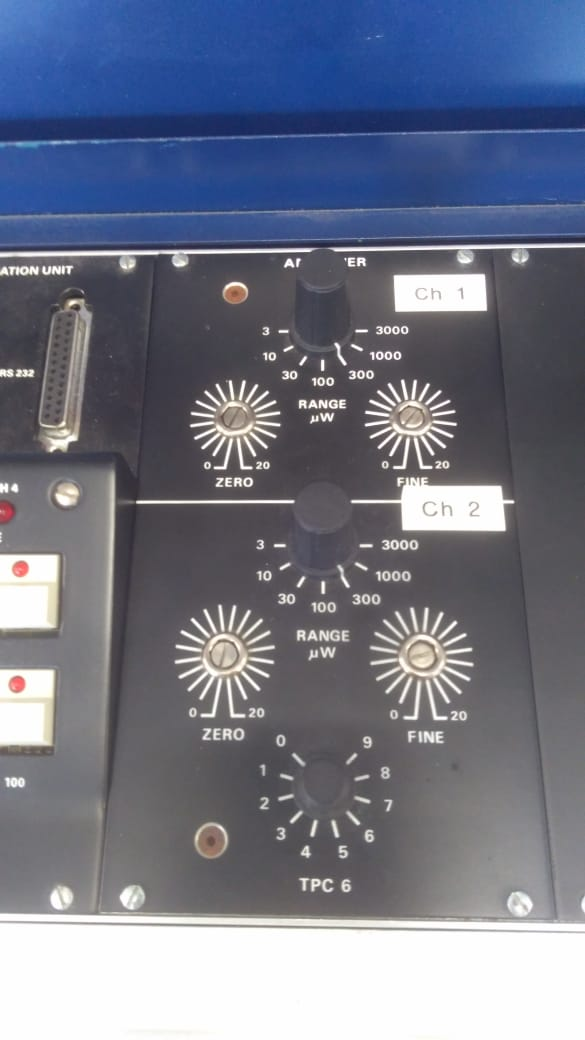
\includegraphics[width=\linewidth]{Figures/process/p4}
			\caption{ }
			\label{fig: subF}
		\end{subfigure}
		\caption{Proceso de instalación de un cilindro de medición.}
		\label{fig: instalationMultiple}
	\end{figure}

	Una vez instalado el cilindro se adicionaron cerca de 25 litros de agua al calor\'imetro usando uno de los orificios que se observa en la \autoref{fig: subC}, y se conectaron las mangueras del baño externo al equipo, cuya conexión se encuentra en la parte inferior del lado izquierdo del calorímetro. Donde el flujo de entrada corresponde con la manguera derecha. Posteriormente el sistema fue encendido y se verific\'o que este registrara la temperatura del ba\~no interno, el valor de la temperatura fue corroborado usando un term\'ometro de mercurio con longitud de 76 mm y nitr\'ogeno gaseoso en su interior, cuyas temperaturas de trabajo se encuentran entre -1,0 \grad{} a 51,0 \grad{} y precisión de 0,1 \grad{} (referencia \texttt{SAMA-CP40-N16B}), encontr\'andose que el calor\'imetro registra una temperatura 0,1 \grad{} superior a aquella medida por el term\'ometro de mercurio.
	
	La conexión con el computador se realiza usando el puerto RS232, que trae el calorímetro, y un conversor de protocolo RS232 a USB. De manera similar se realiza la comunicación con el controlador de la bomba de la jeringa, siendo este el único equipo que no fue posible adaptar a la red eléctrica colombiana, pues su voltaje de operaci\'on es \'unico, por lo cual, su uso requiere de un transformador eléctrico de 110 VAC a 230 VAC. Para el agitador originalmente era necesario el uso de un adaptador de 230 VAC a 5 VDC, pero dado que el voltaje que provee un puerto USB corresponde a este valor, se cambiaron las conexiones de tal forma que ahora solo es necesario conectar el agitador a un puerto de este tipo.
	\begin{figure}[h]
		\centering
		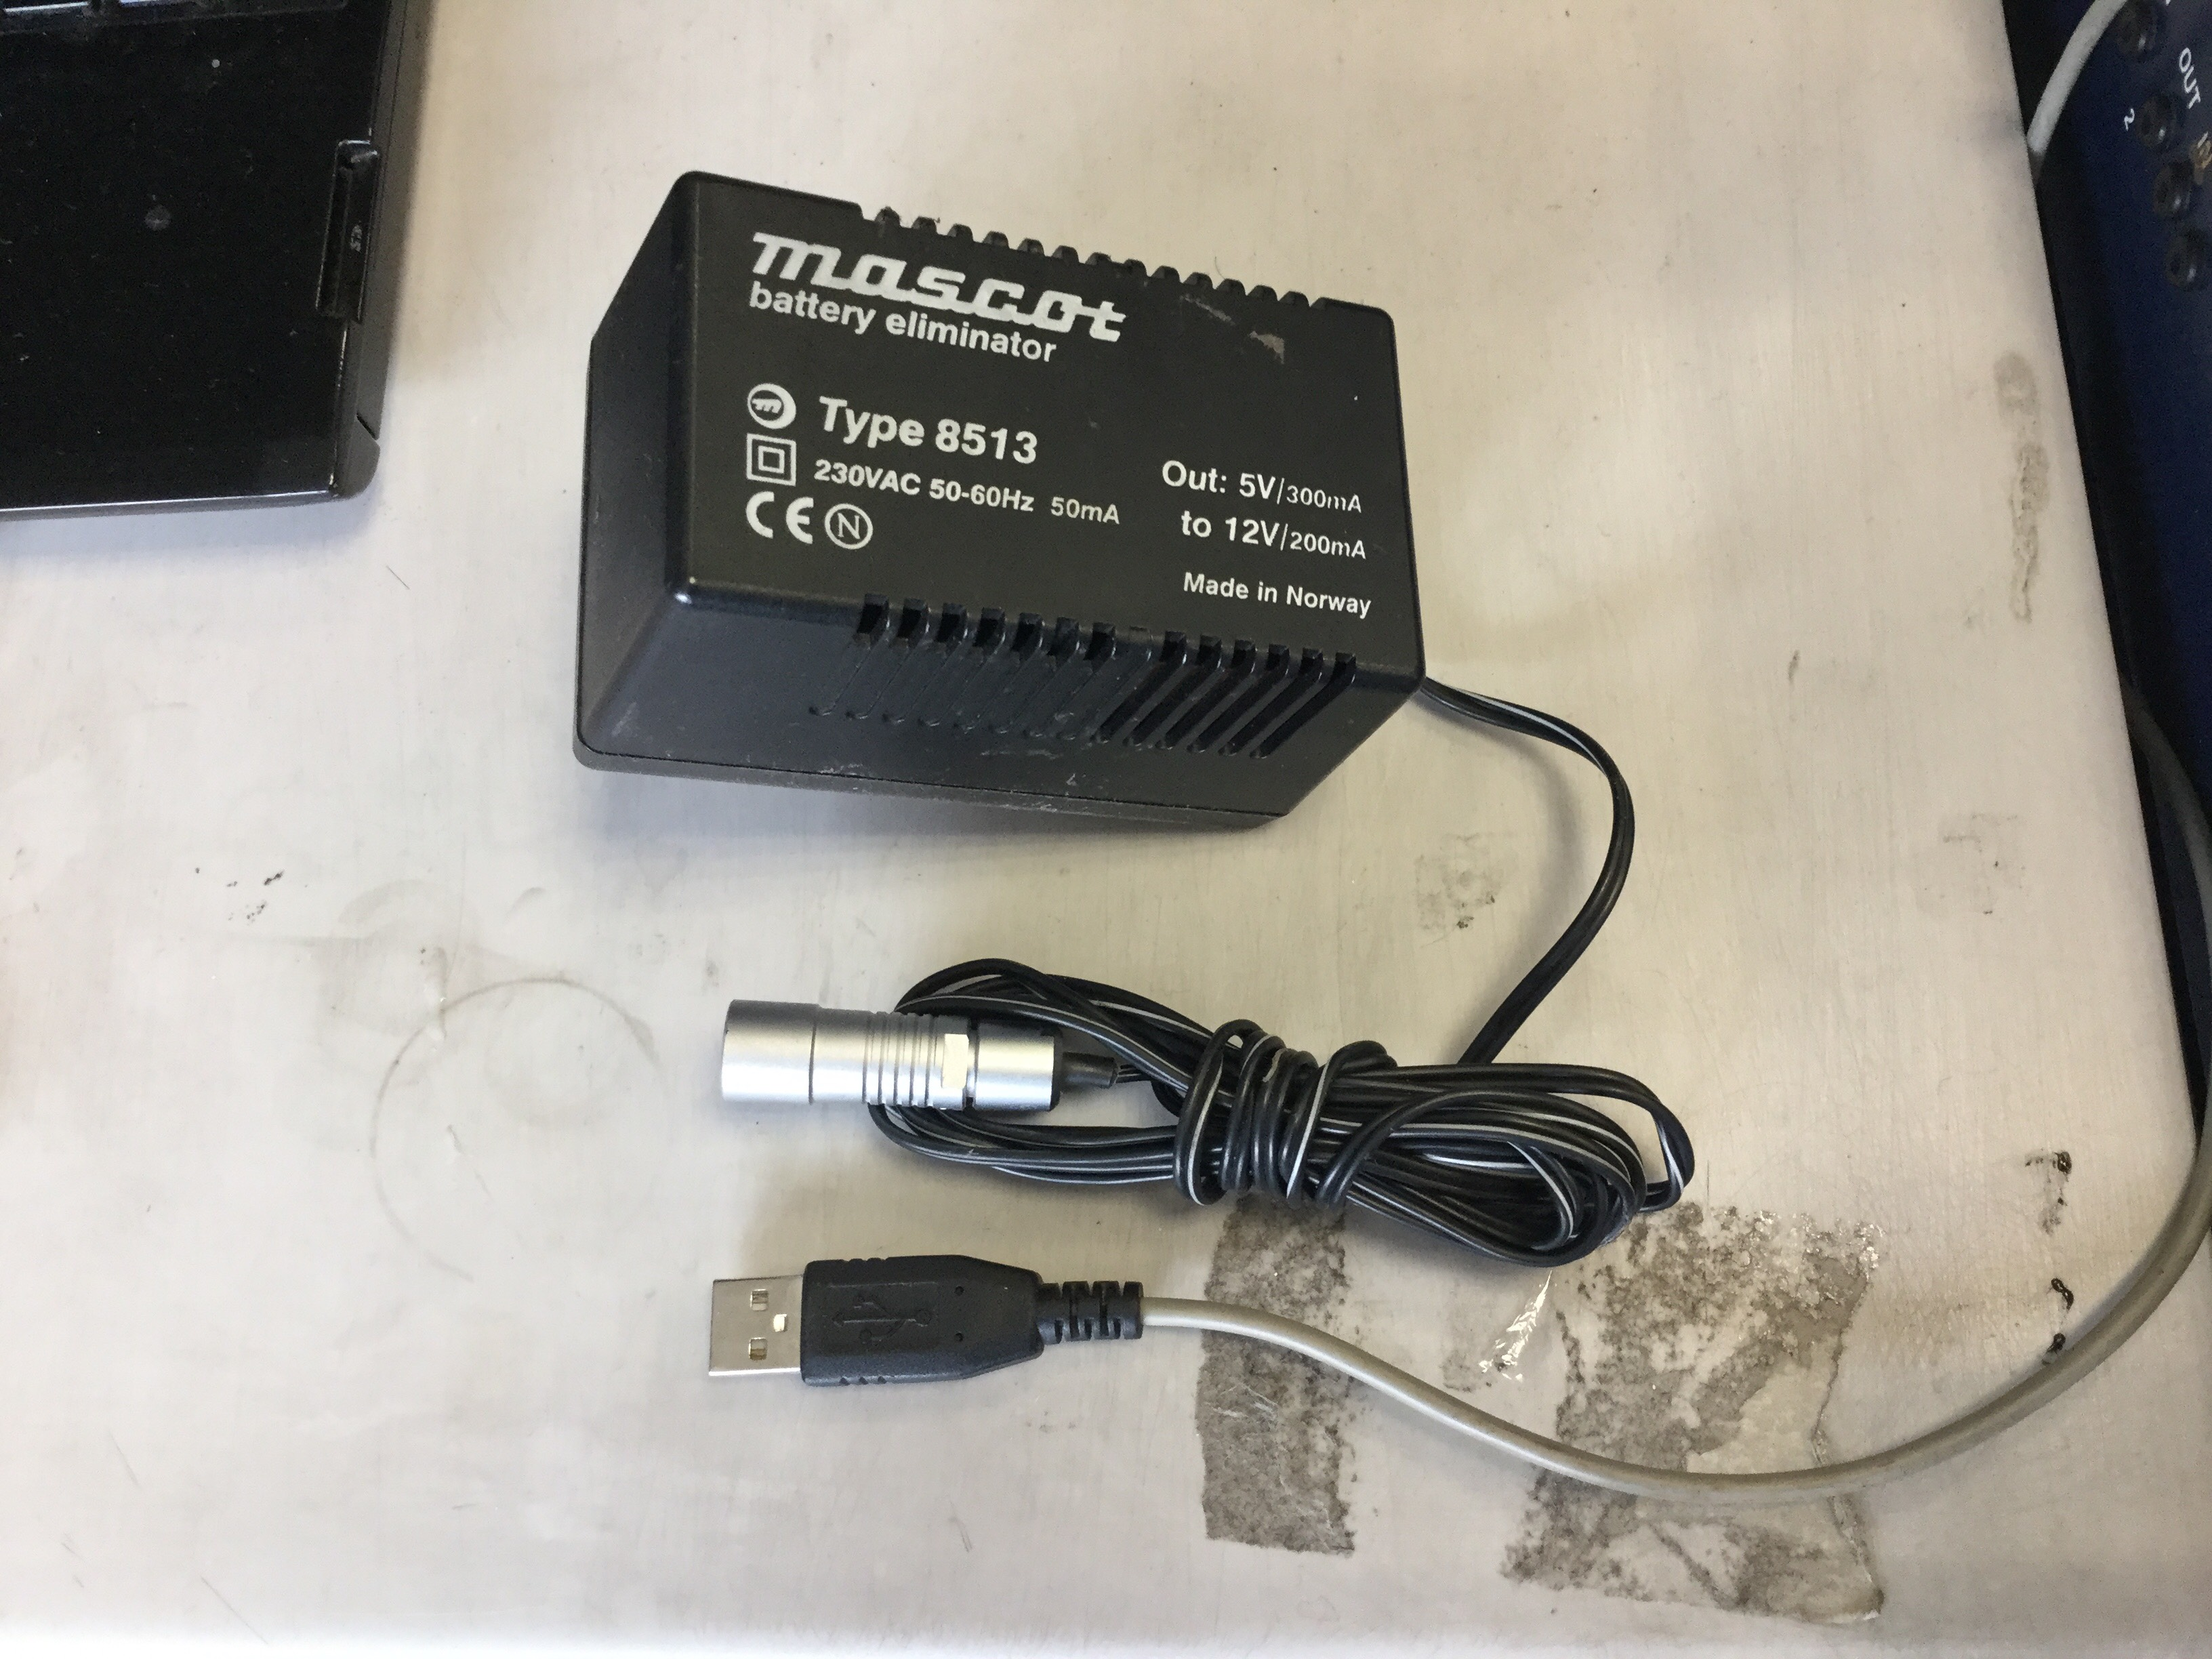
\includegraphics[width=0.5\linewidth]{Figures/motorCircuit}
		\caption{Sistema de alimentaci\'on original del agitador y el nuevo.}
	\end{figure}
	
	\section{Programa de control}
	El calorímetro cuenta con un programa de control con el nombre de Digitam. Este software se encuentra instalado en el computador que fue importado con el equipo, sin embargo, al momento de conectar el computador, no fue posible iniciar el sistema operativo. Usando un cable SATA-USB, se accedió al disco duro y se realizó una copia del mismo. Una aplicación de MS-DOS con el nombre de Digitam 3 se encontró en el mismo y se ejecutó en una maquina virtual con Windows XP y se logr\'o as\'i la comunicación con el calorímetro (\autoref{fig: digitam3}). Sin embargo, esta aplicaci\'on se ejecuta en la consola de Windows, por lo cual carece de interfaz gr\'afica y el uso del cursor es limitado. En el \'ultimo mes se identific\'o otro software el cual sí presenta interfaz gr\'afica y hace la interacci\'on el usuario mucho m\'as c\'omoda \autoref{fig: digitam4}.
	\begin{figure}[h]
		\centering
		\begin{subfigure}{0.45\linewidth}
			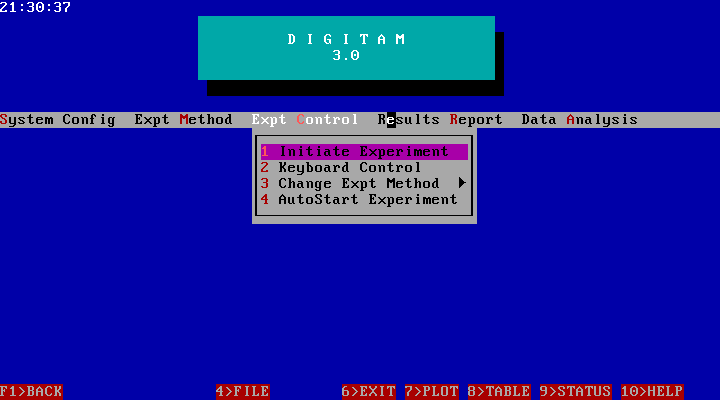
\includegraphics[width=\linewidth]{Figures/digitam}
			\caption{Digitam 3.0}
			\label{fig: digitam3}
		\end{subfigure}
		\begin{subfigure}{0.54\linewidth}
			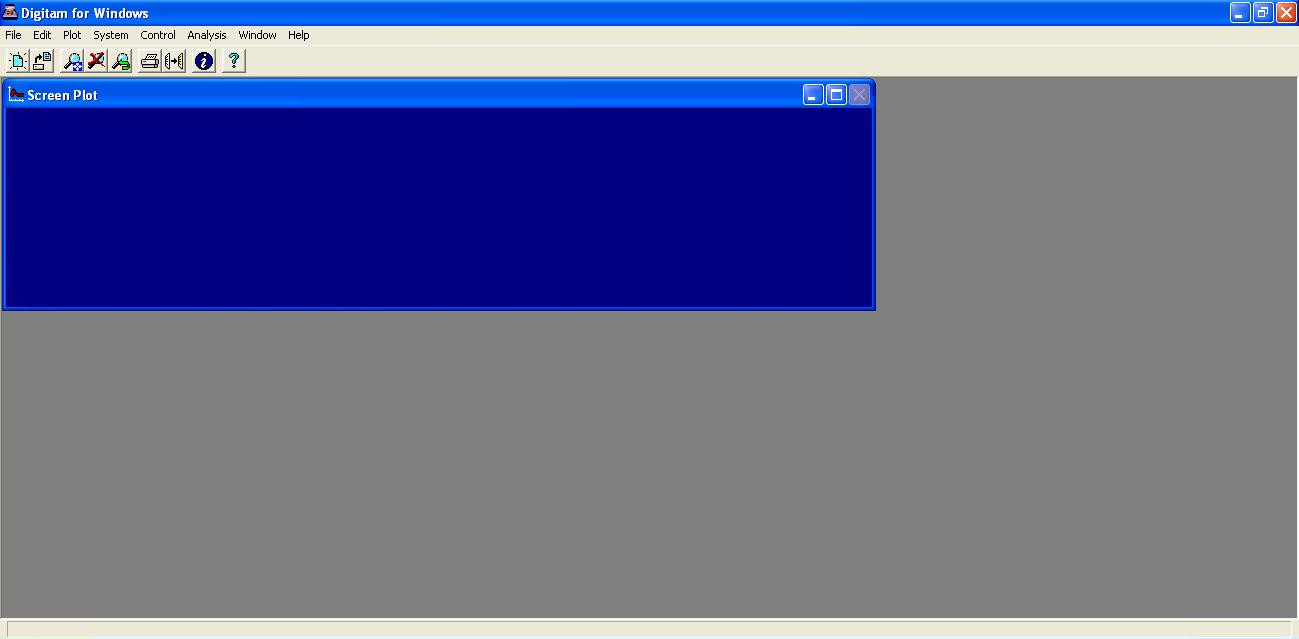
\includegraphics[width=\linewidth]{Figures/digitamView}
			\caption{Digitam 4.0}
			\label{fig: digitam4}
		\end{subfigure}
		\caption{Programas disponibles uso del calor\'imetro con Windows.}
	\end{figure}
	
	\subsection{Configuración del equipo}
	El programa depende de dos directorios en donde guarda los archivos que contienen c\'omo realizar un experimento (m\'etodos) y los resultados. Estos directorios se deben configurar cuando se instala el programa por primera vez y se encuentran en el men\'u principal de Digitam 4 en \texttt{File > Preferences}. En la ventana emergente se debe configurar la ubicaci\'on de los directorios (\texttt{Default results directory} y \texttt{Default method directory}), pues es posible que al iniciar el programa estos no existan por lo cual no sea posible continuar con las siguientes secciones.
	
	\subsection{Creación de un método experimental}
	Como fue mencionado anteriormente, un m\'etodo en Digitam contiene la informaci\'on de qu\'e medir, con qu\'e frecuencia, si se desea inyectar un volumen determinado, realizar el experimento m\'ultiples veces, etc. Para crear un m\'etodo se debe seleccionar \texttt{File > New Method} o si se desea editar uno previo: \texttt{File > Open > Method}. En este punto se debe seleccionar como dividir el experimento, cada parte puede tener hasta cuatro secciones, como es el caso de las opciones 5 \'o 6. Adem\'as, se pueden concatenar hasta 3 partes seguidas, como se muestran en la \autoref{fig: methodCreation}.
	
	Posteriormente, se deben definir las condiciones que determinan un cambio de secci\'on en un una misma parte del m\'etodo. En el caso de \autoref{fig: methodSectionChange} para la tercera parte del experimento, en la secci\'on \texttt{Main}, se define la duraci\'on de este como 60 minutos, en el caso de usar las condiciones de estabilidad se debe expandir la opci\'on de \texttt{Section change condition} en el panel superior izquierdo, y definir las condiciones en \texttt{Signal conditions}.
	\begin{figure}[h]
		\centering
		\begin{subfigure}{0.45\linewidth}
			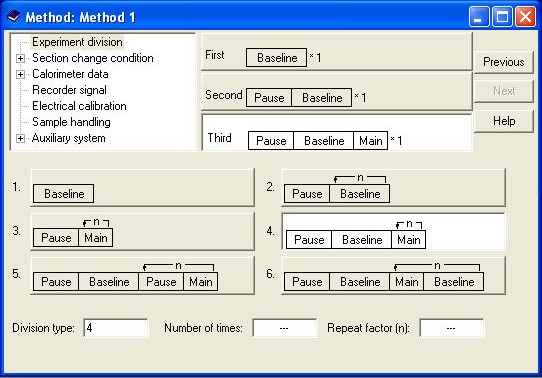
\includegraphics[width=\linewidth]{Figures/digitamMethod}
			\caption{Definici\'on de las partes y secciones de un m\'etodo.}
			\label{fig: methodCreation}
		\end{subfigure}
		\begin{subfigure}{0.45\linewidth}
			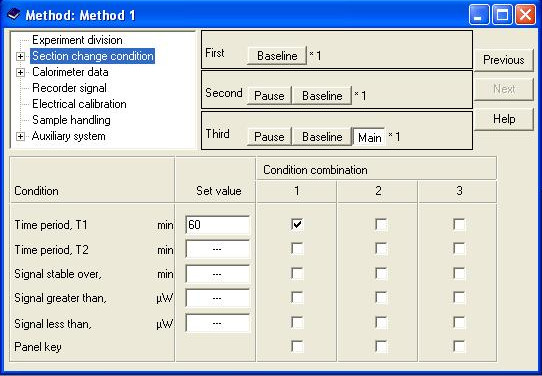
\includegraphics[width=\linewidth]{Figures/digitamMethod2}
			\caption{Configuraci\'on de las condiciones para cambiar de secci\'on.}
			\label{fig: methodSectionChange}
		\end{subfigure}
		\caption{Paneles de creaci\'on y modificaci\'on de un m\'etodo, configuraci\'on del mismo.}
		\label{fig: methodPanel}
	\end{figure}
	
	En \texttt{Calorimeter data} se escoge la frecuencia con la que se muestrea la se\~nal del calor\'imetro, si se quiere promediar la se\~nal a lo largo de cierto intervalo de tiempo, si se quiere filtrar digitalmente (usando las propiedades en \texttt{System > Calorimeter signal > Digital filter}) y si se quiere guardar la se\~nal din\'amicamente corregida. Al igual que en la \autoref{fig: methodSectionChange}, esta configuraci\'on es independiente para cada secci\'on del experimento. Por ejemplo, se puede medir la se\~nal de la primera parte en la secci\'on de \texttt{Baseline} cada segundo sin filtrar la se\~nal (\texttt{raw}), en la segunda parte, en \texttt{Pause} se puede medir la se\~nal corregida y en \texttt{Baseline} medir la potencia pero ahora cada 10 segundos.
	
	Las calibraciones el\'ectricas se configuran en \texttt{Electrical calibration} en el mismo panel de la \autoref{fig: methodPanel}. En ella se debe seleccionar el tipo (\texttt{D} para una calibraci\'on din\'amica y \texttt{S} para una est\'atica, las cuales ser\'an explicadas en el \autoref{sec: electrica}), la potencia, que debe ser del mismo valor del amplificador del canal en el calor\'imetro (300 $\mu$W en el caso de la \autoref{fig: instalationMultiple}) \cite{Suurkuusk}, el tiempo, el cual se debe configurar \'unicamente para el caso de una calibraci\'on est\'atica y se recomienda que sea superior a 30 minutos \cite{Suurkuusk}. En general, el lado de la calibraci\'on es: \texttt{A} para la muestra y \texttt{B} para la celda de referencia \cite{Suurkuusk}, y la resistencia interna, que en el caso de los cilindros usados siempre es permanente \texttt{P}.
	
	La configuraci\'on de los vol\'umenes de inyecci\'on y los tiempos desde el programa, para el caso de titulaciones calorimétricas se describen en la \autoref{ssec: jeringa}. Una vez configurado el método, se debe guardar seleccionando \texttt{File > Save method}.
	
	\subsection{Control del experimento}
	Una vez se ha guardado el experimento, y se desea ejecutar el mismo, se accede al panel de comienzo del experimento. En \'el se debe seleccionar los nombres con los que se desean guardar los resultados, el m\'etodo experimental a usar, y el nombre del operario. Se debe verificar que la configuraci\'on de amplificaci\'on corresponde con la que tiene el canal en el calor\'imetro, y si se realizar\'an inyecciones en una titulaci\'on, el n\'umero del controlador de la jeringa, que en este caso corresponde con \texttt{1}.
	
	\subsection{Configuración de la gráfica}
	Digitam 4 ofrece la posibilidad de graficar los resultados en tiempo real, para esto se debe configurar la gr\'afica. Al acceder a \texttt{Plot > Define Screen Plot} se escribe el nombre de los resultados a graficar, se definen las escalas de la gr\'afica, y el tipo de datos a usar (corregidos, filtrados u originales). Adicionalmente se puede optimizar el \'area de la gr\'afica para que muestre la totalidad de los datos, oprimiendo \texttt{Plot > Scale to Show All}.
	
	\subsection{Extracci\'on los resultados}
	Finalmente, y con el objetivo de exportar los resultados se debe oprimir en el men\'u superior \texttt{File > Open > Results file} y seleccionar el archivo de resultados que se desea abrir. Posteriormente, se debe navegar sobre el diagrama de \'arbol en donde se muestran los par\'ametros de cada secci\'on del m\'etodo experimental. En particular, para obtener los datos registrados por el calor\'imetro se selecciona \texttt{Numeric data} y luego en \texttt{Tabulated}. Luego, se debe ir al men\'u superior y oprimir \texttt{File > Export}, en el dialogo \texttt{Results Report} seleccionar \texttt{Generate numeric data report for table import}, seleccionar las columnas a incluir y elegir el nombre del archivo de salida.
	
	El archivo de salida puede ser le\'ido en Excel, importando los datos con la opci\'on \texttt{Desde texto} en la ventana \texttt{Datos}. La informaci\'on del calor\'imetro se encuentra tabulada con \texttt{Tabs} como delimitador de cada valor, y en la opci\'on de \texttt{origen del archivo} se puede seleccionar \texttt{Wndows ANSI}. Al finalizar este procedimiento los datos pueden ser visualizados en la hoja de c\'alculo.
	
	\section{Efecto del agitador en las lecturas}
	Para comprobar el efecto del agitador en la potencia registrada por el equipo se llevaron a cabo 6 ciclos de conexión-desconexión con 15 minutos entre cada perturbación al sistema, horas después de haber realizado una calibración estática. Las diferencias de potencia generadas entre cada conexión (izquierda) y desconexión (derecha) se muestran en la \autoref{tb: connection}, y en la \autoref{fig: connection}, donde se observan como aumentos y descensos súbitos en la potencia registrada.
	\begin{table}[h]
		\centering
		\caption{Efectos inmediatos de conectar y desconectar el agitador.}
		\begin{tabular}{cc|l|cc|l}
			\hline
			\textbf{Antes ($\mu$W)} & \textbf{Después ($\mu$W)} &  $\Delta$ ($\mu$W) &  \textbf{Antes ($\mu$W)} & \textbf{Después ($\mu$W)} &  $\Delta$ ($\mu$W) \\
			\hline
			-7,58 & -5,5 & 2,08 & -5,84 & -7,78 & -1,94 \\
			-6,12 & -3,78 & 2,34 & -5,12 & -7,04 & -1,92 \\
			-5,04 & -2,76 & 2,28 & -4,17 & -6,48 & -2,31 \\
			-5,43 & -3,21 & 2,22 & -5,22 & -7,31 & -2,09 \\
			-6,65 & -4,72 & 1,93 & -6,71 & -8,54 & -1,83 \\
			-7,75 & -5,84 & 1,91 & -8,35 & -9,93 & -1,58 \\
			\hline
			 & \textbf{promedio} ($\mu$W) & 2,1 $\pm$ 0,2 & & & -1,9 $\pm$ 0,2 \\
			\hline
		\end{tabular}
		\label{tb: connection}
	\end{table}

	A partir de los datos de la \autoref{tb: connection} fue posible establecer que el efecto de prender y apagar el agitador es de aproximadamente 2 $\mu$W, siendo un aumento en el caso de conexión y una disminución al desconectarlo. Lo anterior est\'a relacionado con que el agitador realiza trabajo sobre la solución, que al encontrarse en un sistema isotérmico la energía se transmite la energ\'ia en forma de calor, y de forma diferencial será registrado como un aumento de potencia en el calorímetro. La \autoref{fig: connection} muestra que este efecto es local en el tiempo y que el sistema tiende a equilibrarse nuevamente al valor de la línea base. Esto se explica ya que el sistema luego de registrar el aumento súbito experimenta una disminución de la potencia lenta, lo contrario ocurre con la desconexión, por lo cual el sistema tiende a retomar el equilibrio dado por la curva naranja, la cual se obtiene realizando mínimos cuadrados con los datos sobre un polinomio de grado 2.
	\begin{figure}[h]
		\centering
		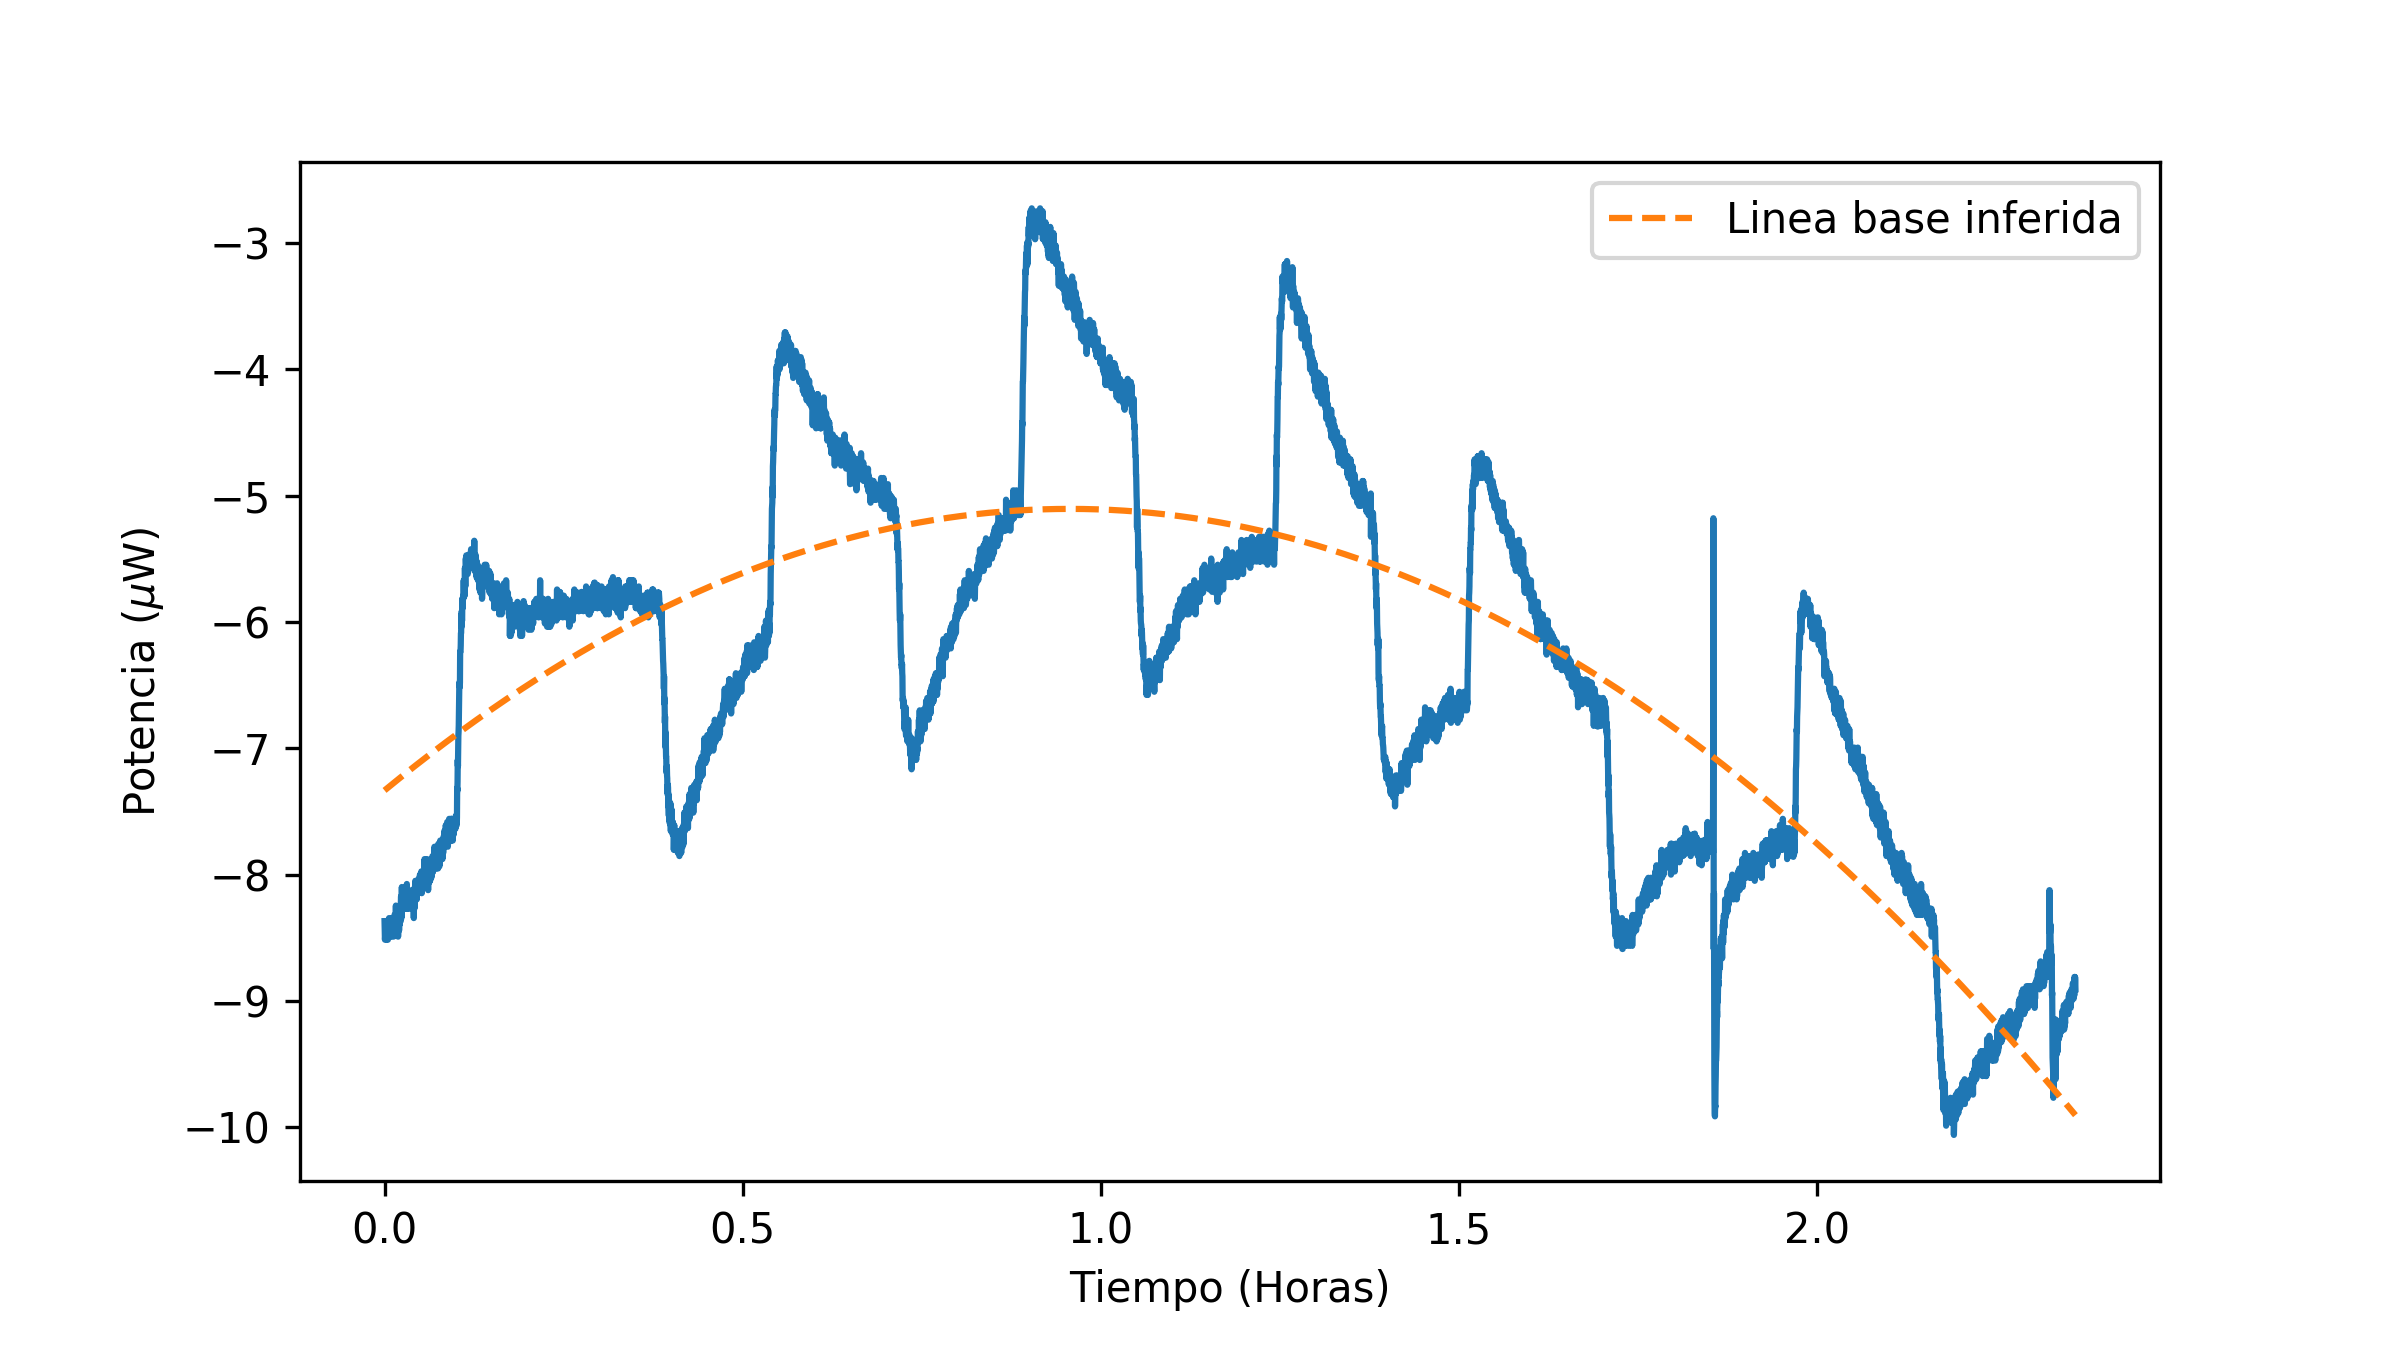
\includegraphics[width=\linewidth]{../Data/Baselines/motor}
		\caption{Conexiones y desconexiones del agitador que perturban la línea base, sin embargo, lentamente el equipo vuelve al equilibrio.}
		\label{fig: connection}
	\end{figure}	